%
%\noindent
%\epigraph{But now they drift on the still water, \\
%Mysterious, beautiful; \\
%Among what rushes will they build, \\
%By what lake's edge or pool \\
%Delight men's eyes when I awake some day \\
% To find they have flown away?}{\textit{W.B. Yeats}}

In addition to $X_{88}$ and $X_{100}$, a gaggle of 50+ other TCs are also known to lie on the EB \cite[X(9)]{etc}, e.g., $X_{162}$, $X_{190}$, $X_{651}$, etc. We have found experimentally that the motion of $X_{100}$ and $X_{190}$ is always monotonic.

In contradistinction: Let $\alpha_{162}{\simeq}1.1639$ be the only positive root of $5 x^8 + 3 x^6 - 32 x^4 + 52 x^2 - 36$.

\begin{proposition}\label{prop:x162}
The motion of $X_{162}$ with respect to $P_1(t)$ is non-monotonic if $a/b>\alpha_{162}$. 
\end{proposition}

\begin{proof}
The trilinear coordinates of $X_{162}$ are given by
{\small 
\[  \frac {1}{ \left( s_2^{2}-  s_3^{2} \right)  \left( s_2^{2}+ s_3^{2}-
s_1^{2} \right) } :  \frac {1}{ \left( s_3^{2}-  s_1^{2} \right)  \left( s_3^{2}+ s_1^{2} -
s_2^{2} \right) }:\frac {1}{ \left( s_1^{2}-  s_2^{2} \right)  \left( s_1^{2}+ s_3^{2} -
s_3^{2}\right) }\cdot
\]
}
Let a 3-periodic $P_1P_2P_3$ be parametrized by $P_1(t)=(a\cos t, b\sin t)$, with $P_2(t)$ and $P_3(t)$
given in Appendix \ref{app:vertices}.
% See\cite{garcia2019-incenter}.
Using the trilinear coordinates above, we have   $X_{162}(t)=(x_{126}(t), y_{126}(t))$ 
  At $t=\frac{\pi}{2}$, $P_1=(0,b)$ and   $X_{162}(\frac{\pi}{2})= (0,b)$.
  
  Solve $x_{162}'(t)|_{t=\frac{\pi}{2}}=0$ for $a/b$. After some long algebraic symbolic manipulation, this is equivalent to solving $5 x^8 + 3 x^6 - 32 x^4 + 52 x^2 - 36=0$, whose positive roots is $  \alpha_{162} \simeq 1.16369.$
\end{proof}

Since $\alpha_{88}>\alpha_{162}$, settting $a/b>\alpha_{88}$ implies both centers will move non-monotonically.

If the EB be a lake, their joint motion is a dance along its margins.
Over a complete revolution of $P_1(t)$ around the EB, $X_{88}$ and $X_{162}$ wind thrice around it, however:

\begin{proposition}
$X_{88}$ and $X_{162}$ never coincide, therefore their paths never cross each other.
\end{proposition}

\begin{proof}
Consider an elementary triangle $P_1=(-1,0)$, $P_2=(1,0)$ and $P_3=(u,v).$
Obtain cartesian coordinates for $X_{88}$ and $X_{162}$ using their trilinears (propositions \ref{prop:x88} and \ref{prop:x162}). The equation $X_{88}=X_{162}$ is given by two algebraic equations $F(u,v,s_1,s_2)=G(u,v,s_1,s_2)=0$ of degree 17 with   $s_1=\sqrt{(u-1)^2+v^2}=\mid P_3-P_2\mid$ and $s_2=\sqrt{(u+1)^2+v^2}=\mid P_2-P_1\mid$.
Particular solutions of these equations are    equilateral triangles with $P_3=(0,\pm \sqrt{3}).$ 
Analytic and  graphic analysis reveals that the level curves $F=G=0$ are as shown in Figure~\ref{fig:x88x162}.

Therefore the equilateral triangle is the only one such that    the triangle centers $X_{88}$ and $X_{162}$ are equal.  It is well known that an equilateral billiard orbit occurs only  when the billiard ellipse is a circle. This ends the proof.
%\textcolor{red}{sketch. A figura esta com %cores erradas. Vou corrigir mas nao consigo %agora pois o meu inkscape nao funciona mais %com a atualizacao do mac.}
\end{proof}

Their never-crossing joint motion as well as the instants when they come closest is illustrated in Figure~\ref{fig:flat-torus}.

\begin{figure}[H]
    \centering
    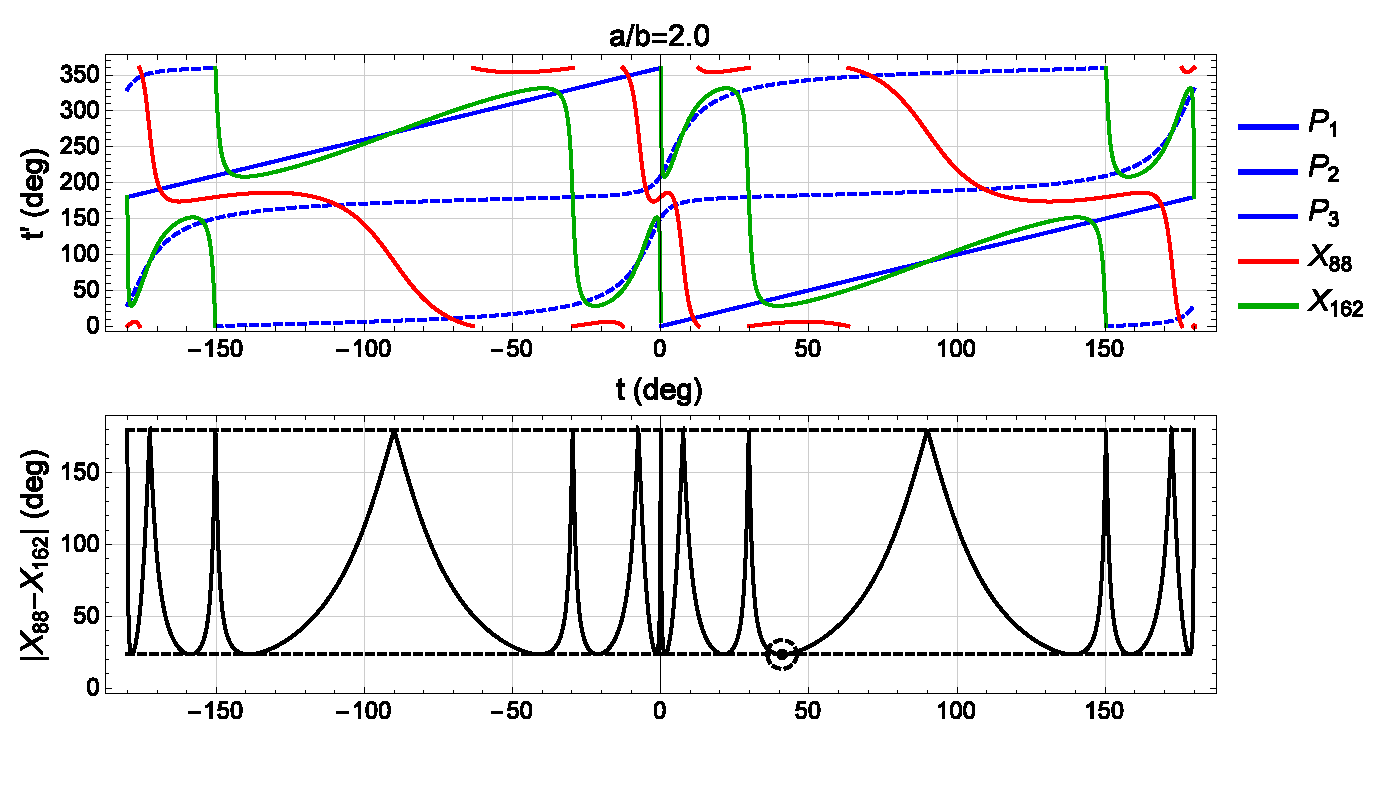
\includegraphics[width=\textwidth]{pics/1150_flat_torus_x88_x126.eps}
    \caption{\textbf{Top}: location $t'$ of 3-periodic vertices $P_1$ (blue), $P_2$ (dashed blue), and $P_3$ (dashed blue), as well as $X_{88}$ (red), and $X_{162}$, plotted against the $t$ parameter of $P_1(t)$. \textbf{Bottom}: absolute parameter difference along the EB between $X_{88}$ and $X_{162}$. Notice there are 12 identical maxima at $180^\circ$ occurring when the two centers at the left and right vertices of the EB. Additionally, there are 12 identical minima whose values can be obtained numerically. The fact that the minimum is above zero implies the points never cross. Note the highlighted minimum at $t{\simeq}41^\circ$: it is referred to in Figure~\ref{fig:3d-torus}.}
    \label{fig:flat-torus}
\end{figure}

These paths can also be viewed as non-intersecting loops on the torus shown in Figure~\ref{fig:3d-torus}. An animation of this intricate motion can be viewed in  \cite[PL\#14]{reznik2020-playlist-intriguing} with triangle centers imagined as swans.

\begin{figure}
    \centering
    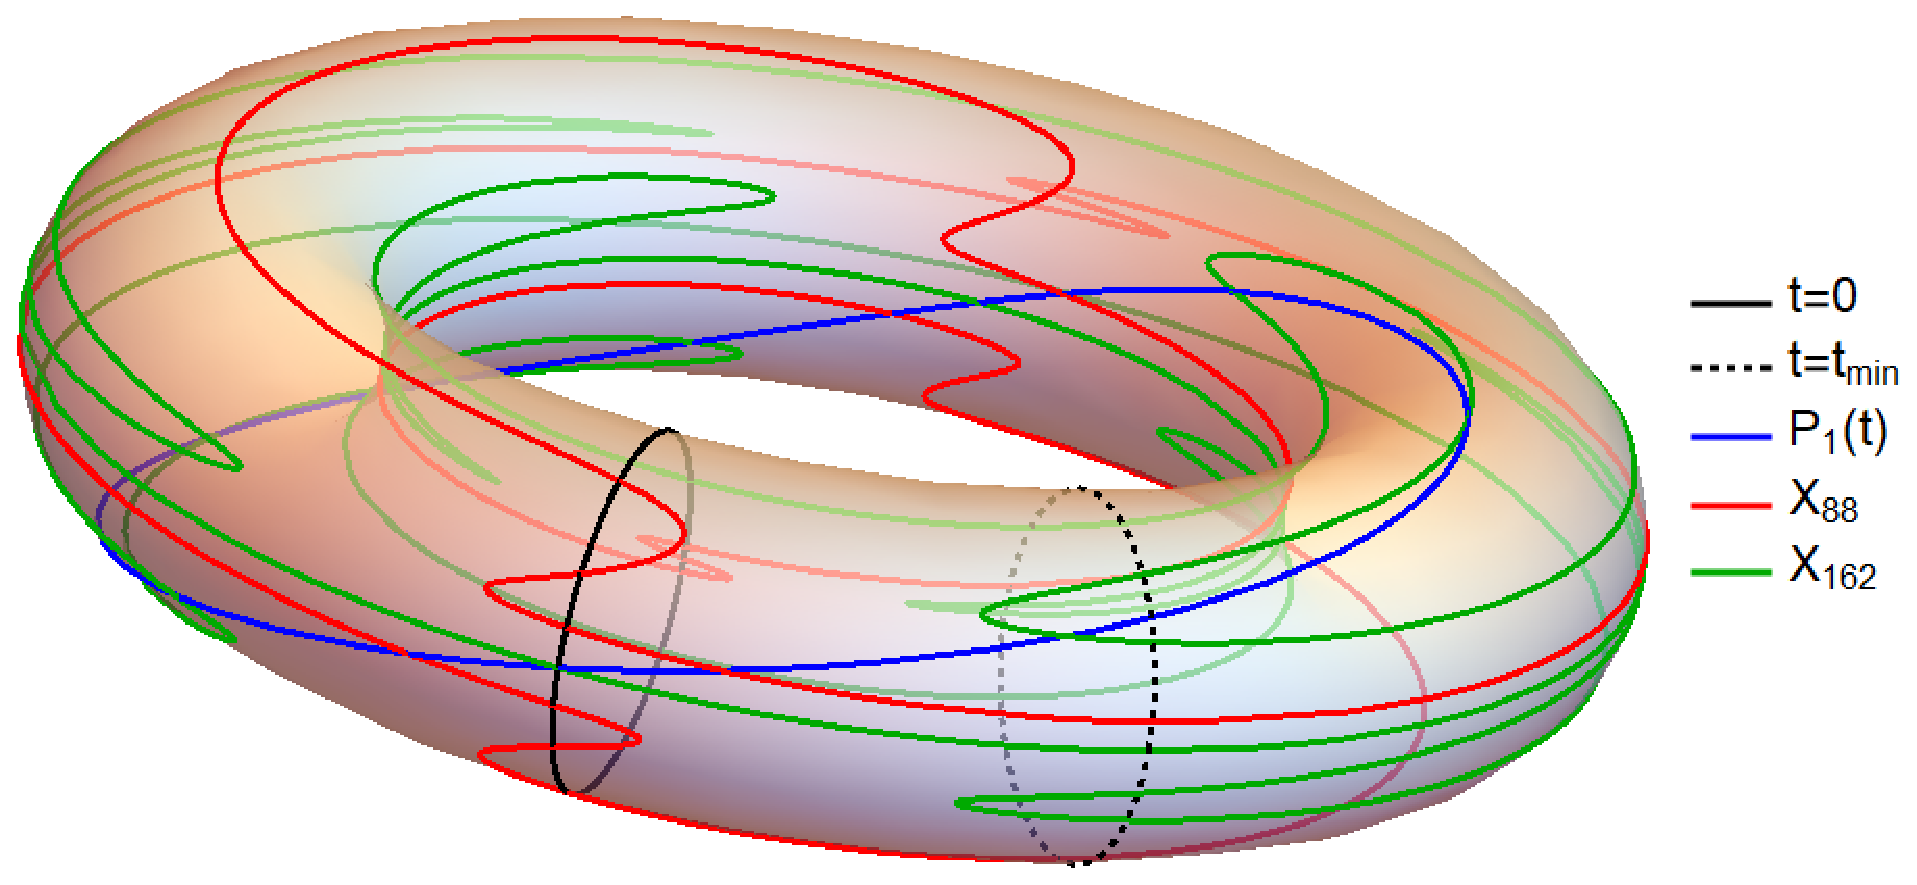
\includegraphics[width=.75\textwidth]{pics/1160_torus_x88_x126_cropped.eps}
    \caption{Visualizing the joint motion of $P_1(t),X_{88},X_{162}$ on the surface of a torus. The meridians (circles around the smaller radius) correspond to a given $t$ (a solid black meridian is wound at $t=0$. The parallels represent a fixed location on the Billiard boundary. The curves for $X_{88}$ and $X_{162}$ are thrice-winding along the torus though never intersecting. To be determined: an analytic value for $t$ where $X_{88}$ and $X_{162}$ are closest (there are 12 solutions). The dashed meridian represents one such minimum which for $a/b=2$ occurs at $t{\simeq}41^\circ$. Notice it does not coincide with any critical points of motion.}
    \label{fig:3d-torus}
\end{figure}

%\begin{figure}
%    \centering
%    \includegraphics[width=\linewidth]{1200_pics_swan_frames}
%    \caption{Triangle Center Ballet along the margins of an $a/b=2.5$ Elliptic Lake. (i) while $P_1$ moves CCW, Triangle Swanters $X_{88}$ and $X_{162}$ glide toward each other; (ii) at their closest they touch bills. (iii) Suddenly, $X_{162}$ reverses course, (iv) and a short-lived same-direction pursuit ensues. (v) An unswooned $X_{88}$ also changes course, (vi) and now both glide in opposite directions. The duo will meet again on 2nd, 3rd and 4th quadrants, where the dance steps are played back in alternating forward and backward order. Clutching to the center of the lake is a black {\em Mittenschwan}. With some help from Tchaikovsky, \textbf{Video}: \cite[PL\#14]{reznik2020-playlist-intriguing}}
%    \label{fig:x88-x162}
%\end{figure}

Though we lack a theory for non-monotonicity of EB-bound TCs $X_i$, we think it is ruled by at least the following aspects:

\begin{itemize}
    \item When the 3-periodic is an isosceles, will $X_i$ lie at the summit vertex or below the base?
    \item As the 3-periodic rotates about the EB, does $X_i$ follow it or move counter to it?
    \item Can $X_i$ be non-monotonic? For example, neither $X_{100}$ nor $X_{190}$ ever are. If so, what is the aspect ratio $\alpha_i$ which triggers it?
\end{itemize}

Still murky is how the above derive from the Trilinears which specify $X_i$. We refer the reader to an animation depicting the joint motion of 20-odd such centers \cite[PL\#15]{reznik2020-playlist-intriguing}.